\chapter{Fusione e fissione nucleare}
\section{Fissione nucleare}
Negli anni '30 i ragazzi di via Palisperna fanno esperimenti in cui si accorgono che, bombardando con 
neutroni terminci, si possa indurre radioattività: senza accorgersene avevano scoperto il 
fenomeno della fissione indotta.\\
Solo successivamente, in Germania, si accorsero che bombardando Uranio si ottenevano atomi
con A e Z di circa la metà.\\
Prendiamo dunque la reazione:
\begin{align*}
    X^{A}_{Z} \rightarrow Y^{A/2}_{Z/2} + Y^{A/2}_{Z/2}
\end{align*}
calcoliamoci il Q:
\begin{align*}
        Q &= M_{X}-2M_{y}\\
          &= -B_{x}+2B_{y}\\
          &=-7.5A + 2\frac{A}{2}8.5\\
          &\sim 200MeV \tag*{Per atomi pesanti}
\end{align*}
dove abbamo scritto la massa di un nucleo come la somma dei nucleoni meno l'energia di ionizzazione B.\\
Notiamo che Q è molto grande, ad atomi pesanti dunque conviene dividersi in atomi più leggeri,
i 200MeV di differenza finirà in energia cinetica dei due atomi.
\subsection{Cosa succede all'atomo durante la fissione}
Possiamo immaginare che il nucleo, durante il processo, cominci ad allungarsi ellitticamente
\newpage
\begin{figure}[!h]
    \centering
    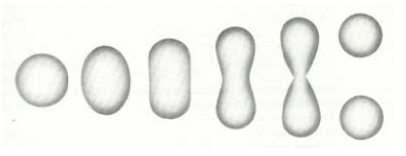
\includegraphics[scale=0.5]{ch6InterazioneMateria/NucleoFissione}
    \caption{Nucleo che si sta separando}
\end{figure}

All'interno del nucleo abbiamo visto (modello a goccia) che vi sono termini di interazione fra i 
nucleoni, in particolare:
\begin{itemize}
        \item Termine di superficie: è il termine che rema contro il legame nucleare, esso 
                in questa separazione sta aumentando:
        \item Termine culombiano : termine, aiuta il legame del nucleo, che dipende dalla distanza fra i protoni, durante la 
                separazione la distanza fra essi aumenta, diminuendo di conseguenza tale termine.
\end{itemize}
Manca l'immagine ma vediamo cosa succede con più esattezza ai termini sopra:
\begin{align*}
    &b_{1}A^{2/3}\rightarrow b_{1}A^{2/3}(1-\frac{2}{5}\epsilon^2)\\[1em]
    &b_{2}\frac{Z(Z-1)}{A^{1/3}}\rightarrow b_{2}\frac{Z(Z-1)}{A^{1/3}}(1-\frac{\epsilon^2}{5})
\end{align*}
Si nota come il primo termine (quello superficiale) aumenta e il secondo (culombiano) diminuisce.\\
A questo punto dobbiamo confrontare le masse dei nuclei nella forma sferica e in quella ellissoidale e
vedere quando la seconda è privilegiata rispetta la prima.
\begin{align*}
        M(sfera)-M(ellissoide) &= -B_{sf}+B_{elis} \\
                               &= -b_{1}A^{2/3}+b_{1}A^{2/3}(1-\frac{2}{5}\epsilon^2)-b_{2}\frac{Z(Z-1)}{A^{1/3}}+b_{2}\frac{Z(Z-1)}{A^{1/3}}(1-\frac{\epsilon^2}{5}
\end{align*}
Questo non è altro che il celeberrimo Q value che abbiamo visto anche nei decadimenti, 
andiamo a vedere quando esso è maggiore o minore di 0:
\begin{align*}
    2b_{1}\frac{Z^2}{A^{1/3}}>< b_{2}\frac{Z^2}{A^{1/3}}\rightarrow \frac{2b_{1}}{b_{2}}><\frac{Z^2}{A}
\end{align*}
Sapendo che $2b_{1}/b_{2}\sim50$ si deduce che non è assolutamente scontato che un atomo faccia
fissione spontaneamente ma tanto più è grande $Z^2/A$ più è probabile che succeda. 
\newpage
\subsection{Fissione nucleare indotta}
Per spiegare la fissione indotta ci concentriamo sui nuclei $U^{235}_{92}$ e $U^{238}_{92}$, 
seppur la concentrazione del primo sia nettamente inferiore questo ha una importanza straordinaria
e vediamo ora il perchè.
Per avere fissione indotta si ha un neutrone che colpisce il nucleo producendo 2 prodotti di fissione e
2 o 3 neutroni.
\begin{tcolorbox}[colback=red!5!white,colframe=red!50!black,title=ATTENZIONE !]
I prodotti di fissione non sono definiti univocamente, la distribuzione di fissione ha 2 picchi.
\end{tcolorbox}
A livello energetico quello che succede è questo : quando un U 235 viene colpito da un neutrone 
termino si crea un nucleo $U^{236*}$ eccitato, ossia con energia poco superiore a quella del
$U^{236}$.
Ci calcoliamo l'energia di eccitamento:
\begin{align*}
    &M(U^{236*}) = M(U^{235})+n \\
    &E_{ecc} = M(U^{236*})-M(U^{236}) \simeq 6,54MeV 
\end{align*}
Se consideriamo l'energia di soglia per la quale avviene la fissione $E_{sogl}\sim 6MeV$ notiamo che in 
questo caso avviene la fissione.
Studiamo ora il caso del $U^{238}$, il ragionamento è esatamente lo stesso ma si ottiene:
\begin{align*}
    E_{ecc} = M(U^{239*})-M(U^{239}) \sim 4,8MeV
\end{align*}
Il fatto è che U 238 è pari-pari e per il nuclei pari-pari l'energia di legame è più alta,
ciò implica che il neutrone termico non riesce a dare abbastanza energia per eccitare il nucleo e 
dare via alla fissione.
